\let\lesson\undefined
\newcommand{\lesson}{\phantomlesson{Bài 4.}}


\setcounter{section}{2}
\section{Bài tập trắc nghiệm}
\begin{enumerate}[label=\bfseries Câu \arabic*:,leftmargin=1.5cm]
	\item \mkstar{1}\\
	{Hãy chọn câu phát biểu đúng?
	\begin{mcq}
		\item Hệ quy chiếu bao gồm hệ toạ độ, mốc thời gian và đồng hồ.
		\item Hệ quy chiếu bao gồm vật làm mốc, mốc thời gian và đồng hồ.
		\item Hệ quy chiếu bao gồm vật làm mốc, hệ toạ độ, mốc thời gian.
		\item Hệ quy chiếu bao gồm vật làm mốc, hệ toạ độ, mốc thời gian và đồng hồ.
	\end{mcq}
}
\hideall{
\textbf{Đáp án: D.}
}

\item \mkstar{1}\\
{Kết luận nào sau đây là đúng khi nói về độ dịch chuyển và quãng đường đi được của một vật?
	\begin{mcq}
		\item Độ dịch chuyển và quãng đường đi được đều là đại lượng vô hướng.
		\item Độ dịch chuyển là đại lượng vectơ còn quãng đường đi được là đại lượng vô hướng.
		\item Độ dịch chuyển và quãng đường đi được đều là đại lượng vectơ.
		\item Độ dịch chuyển và quãng đường đi được đều là đại lượng không âm.
	\end{mcq}
}
\hideall{
\textbf{Đáp án: B.}
}

\item\mkstar{2}\\
{Một vật bắt đầu chuyển động từ điểm $O$ đến điểm $A$, sau đó chuyển động về điểm $B$. Quãng đường và độ dịch chuyển của vật tương ứng là
	\begin{center}
		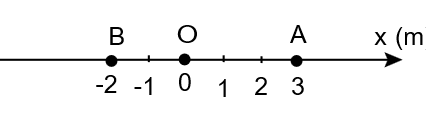
\includegraphics[width=0.4\linewidth]{../figs/VN10-2022-PH-TP004-P-2}
	\end{center}
\begin{mcq}(4)
	\item $\SI{2}{\meter}$; $\SI{-2}{\meter}$.
	\item $\SI{8}{\meter}$; $\SI{-2}{\meter}$.
	\item $\SI{2}{\meter}$; $\SI{2}{\meter}$.
	\item $\SI{8}{\meter}$; $\SI{-8}{\meter}$.
\end{mcq}
}
\hideall{
\textbf{Đáp án: B.}
}
\item \mkstar{2}\\
{Nếu nói “Trái Đất quay quanh Mặt Trời” thì trong câu nói này vật nào được chọn làm mốc
	\begin{mcq}(2)
		\item Cả Mặt Trời và Trái Đất.
		\item Trái Đất.
		\item Mặt Trăng.
		\item Mặt Trời.
	\end{mcq}
}
\hideall{
\textbf{Đáp án: D.}
}

\item \mkstar{2}\\
{“Lúc 15 giờ 30 phút hôm qua, xe chúng tôi đang chạy trên quốc lộ 5, cách Hải Dương 10 km”. Việc xác định vị trí của ô tô như trên còn thiếu yếu tố gì?
	\begin{mcq}(2)
		\item Vật làm mốc.
		\item Chiều dương trên đường đi.
		\item Mốc thời gian.
		\item Thước đo và đồng hồ.
	\end{mcq}
}
\hideall{
\textbf{Đáp án: B.}
}

\item \mkstar{2}\\
{Trong trường hợp nào dưới đây số chỉ thời điểm mà ta xét trùng với số đo khoảng thời gian trôi?
	\begin{mcq}
		\item Một trận bóng đá diễn ra từ 15 giờ đến 16 giờ 45 phút.
		\item Lúc 8 giờ một ô tô khởi hành từ Thành phố Hồ Chí Minh, sau 3 giờ chạy thì xe đến Vũng Tàu.
		\item Một đoàn tàu xuất phát từ Vinh lúc 0 giờ, đến 8 giờ 05 phút thì đoàn tàu đến Huế.
		\item Không có trường hợp nào phù hợp với yêu cầu nêu ra.
	\end{mcq}

}
\hideall{
\textbf{Đáp án: C.}
}


\item \mkstar{2}\\
{Bảng giờ tàu ở bên cho chúng ta biết quãng đường và thời gian mà đoàn tàu SE1 chạy từ ga Huế đến ga Sài Gòn (bỏ qua thời gian tàu đỗ lại các ga) tương ứng là
	\begin{center}
		\begin{tabular}{|c|c|c|}
			\hline
			\thead{Tên ga} & \thead{km} & \thead{SE1}\\
			\hline
			Hà Nội & 0 & 22:15\\
			\hline
			Thanh Hoá & 175& 01:28 (ngày $+1$)\\
			\hline
			Huế & 688 & 11:08 (ngày $+1$)\\
			\hline
			Sài Gòn & 1726 & 06:32 (ngày $+2$)\\
			\hline
		\end{tabular}
	\end{center}
	\begin{mcq}(2)
		\item $\SI{1726}{\kilo\meter}$, 4 giờ 36 phút.
		\item $\SI{1726}{\kilo\meter}$, 19 giờ 24 phút.
		\item $\SI{1038}{\kilo\meter}$, 19 giờ 24 phút.
		\item $\SI{1038}{\kilo\meter}$, 4 giờ 36 phút.
	\end{mcq}

}
\hideall{
\textbf{Đáp án: C.}
}

\item \mkstar{3}\\
{\begin{minipage}[l]{0.65\textwidth}
		Hai người đi xe đạp từ $A$ đến $C$, người thứ nhất đi theo đường từ $A$ đến $B$, rồi từ $B$ đến $C$; người thứ hai đi thẳng từ $A$ đến $C$. Cả hai đều về đích cùng một lúc.\\
		Hãy chọn kết luận \textbf{sai}.
		\begin{mcq}
			\item Người thứ nhất đi được quãng đường $\SI{8}{\kilo\meter}$.
			\item Độ dịch chuyển của người thứ nhất và người thứ hai bằng nhau.
			\item Độ dịch chuyển và quãng đường đi được của người thứ nhất bằng nhau.
			\item Độ dịch chuyển của người thứ nhất là $\SI{5.7}{\kilo\meter}$, hướng $\SI{45}{\degree}$ Đông – Bắc.
		\end{mcq}
	\end{minipage}
\begin{minipage}{0.35\textwidth}
	\begin{center}
		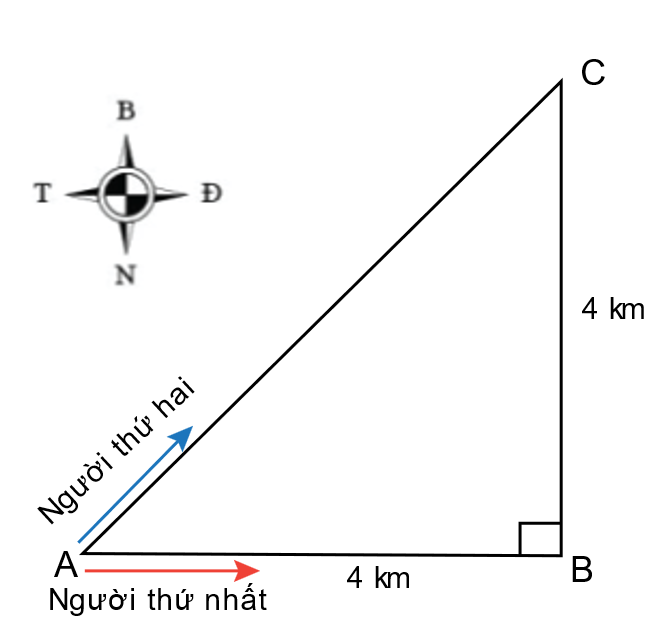
\includegraphics[width=0.7\linewidth]{../figs/VN10-2022-PH-TP004-P-3}
	\end{center}
\end{minipage}

}
\hideall{
\textbf{Đáp án: C.}
}

\item \mkstar{3}\\
{Cho biết Giờ Phối hợp Quốc Tế gọi tắt UTC. So với 0 giờ Quốc Tế, Việt Nam ở múi giờ thứ 7 (UTC+7) và Nhật Bản ở múi giờ thứ 9 (TUC+ 9). Ngày 20/12/2021, máy bay VN300, thuộc hãng hàng không Vietnam Airlines, khởi hành từ Tp. Hồ Chí Minh lúc 0 giờ 20 phút và đến Tp. Tokyo lúc 7 giờ 45 phút, theo giờ địa phương. Thời gian di chuyển của chuyến bay này là
\begin{mcq}(4)
	\item 5 giờ 25 phút.
	\item 9 giờ 25 phút.
	\item 7 giờ 25 phút.
	\item 8 giờ 05 phút.
\end{mcq}
}
\hideall{
\textbf{Đáp án: A.}
}
\item \mkstar{3}\\
{Chuyến bay từ Thành phố Hồ Chí Minh đi Paris khởi hành lúc 21 giờ 30 phút giờ Hà Nội ngày hôm trước, đến Paris lúc 5 giờ 30 phút sáng hôm sau theo giờ Paris. Biết giờ Paris chậm hơn giờ Hà Nội là 6 giờ. Theo giờ Hà Nội, máy bay đến Paris lúc
\begin{mcq}(4)
	\item 11 giờ 30 phút.
	\item 14 giờ.
	\item 12 giờ 30 phút.
	\item 10 giờ.
\end{mcq}
}
\hideall{
\textbf{Đáp án: A.}
}

\end{enumerate}
\section{Bài tập tự luận}
\begin{enumerate}[label=\bfseries Bài \arabic*:,leftmargin=1.5cm]
	\item \mkstar{1}
	
	
	{
		Khi nào quãng đường và độ di chuyển của một vật có cùng một độ lớn?
	}
	
	\hideall
	{	Chuyển động của vật có quỹ đạo là đường thẳng và không đổi chiều chuyển động.
	}

	\item \mkstar{2}
	
	
	{
		Xác định độ dịch chuyển trong các khoảng thời gian liên tiếp bằng nhau của mỗi chuyển động.
		
		\begin{center}
			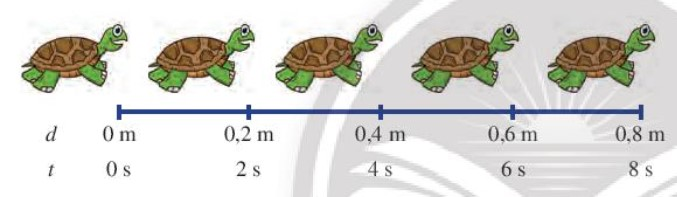
\includegraphics[scale=0.6]{../figs/VN10-2022-PH-TP004-6.jpg}
		\end{center}
	}
	
	\hideall
	{	
		
		Độ dịch chuyển trong các khoảng thời gian liên tiếp bằng nhau của mỗi chuyển động
		
		$$\Delta d_1 = x_2 - x_1 = \SI{0,2}{m}.$$
		
		$$\Delta d_2 = x_3 - x_2 = \SI{0,2}{m}.$$
		
		$$\Delta d_3 = x_4 - x_3 = \SI{0,2}{m}.$$
		
		$$\Delta d_4 = x_5 - x_4 = \SI{0,2}{m}.$$
		
	}


	\item \mkstar{2}
	
	
	{
		Hãy xác định các độ dịch chuyển mô tả ở hình trong tọa độ địa lí.
		
		\begin{center}
			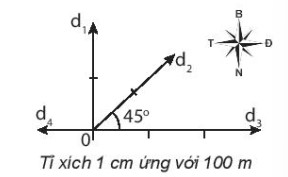
\includegraphics[scale=1]{../figs/VN10-2022-PH-TP004-2.jpg}
		\end{center}
	}
	
	\hideall
	{	
		Độ dịch chuyển mô tả trên hình là:
		
		$+ d_1 = \SI{200}{m}\ \text{(Bắc)}.$
		
		$+ d_2 = \SI{200}{m}\ \text{(Đông Bắc)}.$
		
		$+ d_3 = \SI{300}{m}\ \text{(Đông)}.$
		
		$+ d_4 = \SI{100}{m}\ \text{(Tây)}.$
		
		
	}

	\item \mkstar{2}
	
	
	{
		Một ô tô chuyển động trên đường thẳng. Tại thời điểm $t_1$, ô tô ở cách vị trí xuất phát $\SI{5}{km}$. Tại thời điểm $t_2$, ô tô cách vị trí xuất phát $\SI{12}{km}$. Từ $t_1$ đến $t_2$, độ dịch chuyển của ô tô đã thay đổi một đoạn bằng bao nhiêu?
		
	}
	
	\hideall
	{	
		Từ $t_1$ đến $t_2$ ,  độ dịch chuyển của ô tô thay đổi một đoạn bằng 
		
		$$12-5 = \SI{7}{km}.$$
	}
	\item \mkstar{2}\\
	{Một xe ô tô xuất phát từ tỉnh A, đi đến tỉnh B; rồi lại trở về vị trí xuất phát ở tỉnh A. Xe này đã dịch chuyển, so với vị trí xuất phát một đoạn bằng bao nhiêu? 
	}
	\hideall
	{Xe máy này đã dịch chuyển, so với vị trí xuất phát một đoạn là $\SI{0}{km}$.
	}

	\item \mkstar{2}\\
	{Xác định vị trí của vật A trên trục Ox ở hình vẽ tại thời điểm 12h. Biết vật chuyển động thẳng, mỗi giờ đi được $\SI{40}{km}$.
		
		\begin{center}
			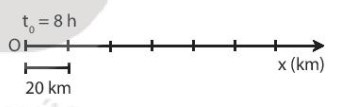
\includegraphics[scale=1]{../figs/VN10-2022-PH-TP004-1.jpg}
		\end{center}
	}
	\hideall
	{	Thời gian vật di chuyển là:
		
		$$12 - 8 = \SI{4}{h}.$$
		
		1 giờ vật di chuyển được $\SI{40}{km}$
		
		$\Rightarrow$ 4 giờ vật di chuyển được: 
		
		$$4 \cdot 40 = \SI{160}{km}.$$
		Tương ứng vật cách gốc toạ độ 8 ô đơn vị.
	}
	
	\item \mkstar{2}
	
	
	{
		Bạn A đi xe đạp từ nhà qua trạm xăng, tới siêu thị mua đồ rồi quay về nhà cất đồ, sau đó đi đến trường. 
		
		\begin{center}
			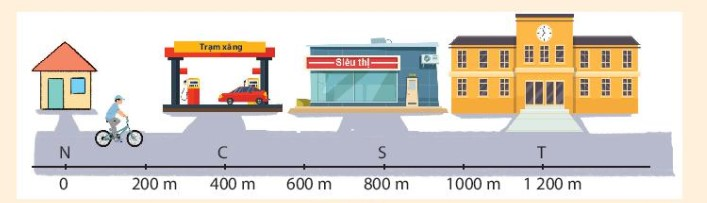
\includegraphics[scale=1]{../figs/VN10-2022-PH-TP004-4.jpg}
		\end{center}
		Chọn hệ tọa độ có gốc là vị trí nhà bạn A, trục Ox trùng với đường đi từ nhà bạn A đến trường. 
		\begin{enumerate}[label=\alph*)]
			\item Tính quãng đường đi được và độ dịch chuyển của bạn A khi đi từ trạm xăng tới siêu thị.
			\item Tính quãng đường đi được và độ dịch chuyển của bạn A trong cả chuyến đi trên.
		\end{enumerate}
	}
	
	\hideall
	{	
		\begin{enumerate}[label=\alph*)]
			\item Quãng đường bạn A đi từ trạm xăng đến siêu thị là: $$800 - 400 = \SI{400}{m}.$$
			
			Độ dịch chuyển của bạn A từ trạm xăng đến siêu thị là: $$800 - 400 = \SI{400}{m}.$$
			
			\item 
			Quãng đường đi được của bạn A trong cả chuyến đi:
			
			+ Quãng đường bạn A đi từ nhà đến siêu thị là: $\SI{800}{m}.$
			
			+ Quãng đường bạn A quay về nhà cất đồ là: $\SI{800}{m}.$
			
			+ Quãng đường bạn A đi từ nhà đến trường là: $\SI{1200}{m}.$
			
			$\Rightarrow$ Quãng đường đi được của bạn A trong cả chuyến đi là: 	$$ 800 \cdot 2 + 1200 = \SI{2800}{m}.$$ 
			
			Điểm đầu xuất phát của bạn A là nhà, điểm cuối của bạn A là trường.
			
			$\Rightarrow$ Độ dịch chuyển của bạn A là $\SI{1200}{m}.$
			
			
			Quãng đường đi được và độ dịch chuyển của A trong cả chuyến đi trên là khác nhau. 
			
		\end{enumerate}
	}
	
	\item \mkstar{2}
	
	
	{
		Hãy so sánh độ lớn của quãng đường đi được và độ dịch chuyển của ba chuyển động. 
		
		\begin{center}
			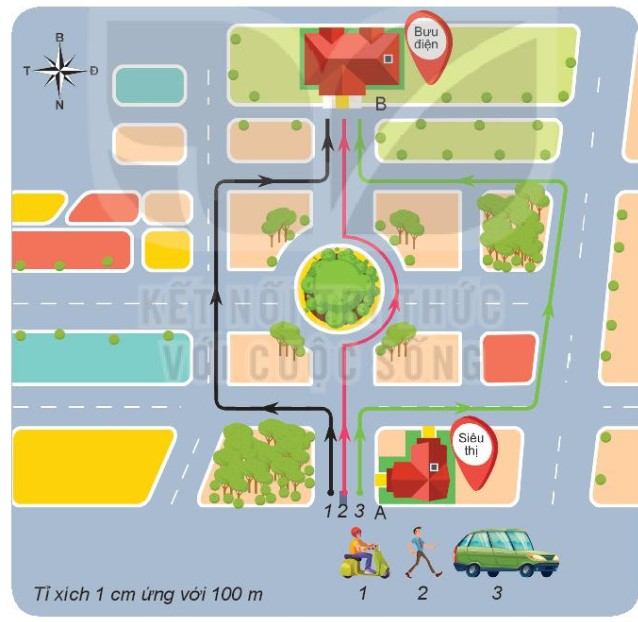
\includegraphics[scale=0.8]{../figs/VN10-2022-PH-TP004-3.jpg}
		\end{center}
	}
	
	\hideall
	{	
		Quãng đường đi được từ ngắn đến dài: $$2 - 1 - 3.$$
		
		Độ dịch chuyển, ta thấy điểm đầu và điểm cuối của ba chuyển động đều như nhau nên độ dịch chuyển của ba chuyển động bằng nhau.
		
	}
	
	
	\item \mkstar{2}
	
	
	{
		Một người lái ô tô đi thẳng $\SI{6}{km}$ theo hướng Tây, sau đó rẽ trái đi thẳng theo hướng Nam $\SI{4}{km}$ rồi quay sang hướng Đông $\SI{3}{km}$. Xác định quãng đường đi được và độ dịch chuyển của ô tô.
	}
	
	\hideall
	{	\begin{center}
			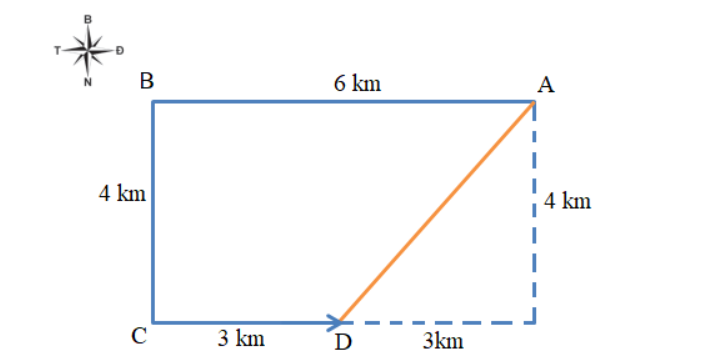
\includegraphics[width=0.4\linewidth]{../figs/VN10-2022-PH-TP004-P-1}
		\end{center}
		Quãng đường đi được :
		
		$$s=6+4+3=\SI{13}{km}.$$
		
		Độ dịch chuyển là :
		
		$$d=\sqrt{3^2+4^2}=\SI{5}{\kilo\meter}$$
	}
	
	
	
\item \mkstar{3}


{
	Một người bơi ngang từ bờ bên này sang bờ bên kia của một dòng sông rộng $\SI{50}{m}$ có dòng chảy theo hướng từ Bắc xuống Nam. Do nước sông chảy mạnh nên khi sang đến bờ bên kia thì người đó đã trôi xuôi theo dòng nước $\SI{50}{m}$. Xác định độ dịch chuyển của người đó.
}

\hideall
{
	\begin{center}
		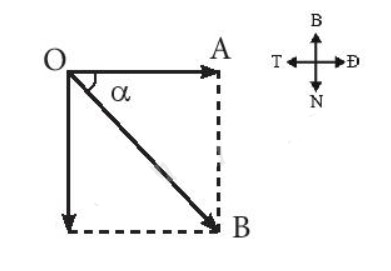
\includegraphics[scale=0.6]{../figs/VN10-2022-PH-TP0001-2.jpg}
	\end{center}
	Người bơi ngang từ bờ bên này sang bên kia theo dự định là OA = $\SI{50}{m}$.
	
	Thực tế, do nước sông chảy mạnh nên vị trí của người đó ở vị trí B, ta có AB = $\SI{50}{m}$.
	
	$\Rightarrow$ Độ dịch chuyển:
	
	$$\Rightarrow\text{OB} = \sqrt{\text{OA}^2 + \text{AB}^2} = \SI{70,7}{km}.$$ 
}
\end{enumerate}